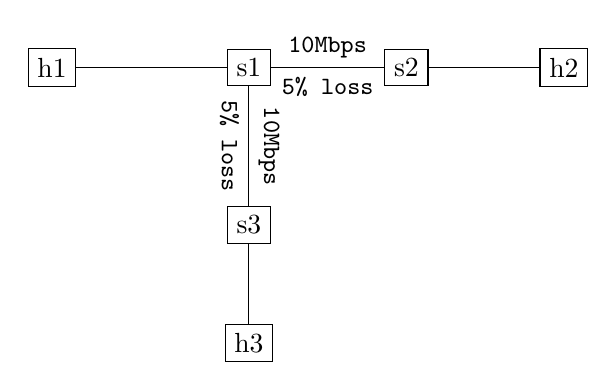
\begin{tikzpicture}
\tikzstyle{host}=[draw]
\tikzstyle{switch}=[draw]
\tikzstyle{connection}=[]
\tikzstyle{constr}=[above,sloped,font=\ttfamily\small]
\tikzstyle{moreconstr} = [constr,below]
\node[host] (h1) at (-0.5,-0.5) {h1};
\node[host] (h2) at (6,-0.5) {h2};
\node[host] (h3) at (2,-4) {h3};
\node [switch] (s1) at (2,-0.5) {s1};
\node [switch] (s2) at (4,-0.5) {s2};
\node [switch] (s3) at (2,-2.5) {s3};
\draw [connection] (h1) edge (s1);
\draw [connection] (s1) edge node[constr] {10Mbps} node[moreconstr] {5\% loss} (s2);
\draw [connection] (s2) edge (h2);
\draw [connection] (s1) edge node[constr] {10Mbps} node[moreconstr] {5\% loss} (s3);
\draw [connection] (s3) edge (h3);
\end{tikzpicture}